\chapter{Einleitung}

In dieser Arbeit soll die Anwendung von Datenanalysen und insbesondere
von \emph{\gls{glos:Predictive_Analytics}} im öffentlichen Sektor untersucht
werden.
Der Schwerpunkt liegt dabei auf Deutschland, wobei aber auch relevante
Anwendungsgebiete in anderen Staaten betrachtet werden. \\ \\
Der einleitende Teil~\ref{part:Schw_Vorhersagen} soll zunächst das Problem der
Schwierigkeit von
Prognosen untersuchen und damit eine Motivation für die Anwendung von 
\emph{predictive analytics} liefern. \\ \\
In Teil~\ref{part:Konzepte_PA} werden die wichtigsten Konzepte von
\emph{predictive analytics} vorgestellt. Dabei werden auch die allgemeinen
Risiken bei der Anwendung diskutiert. \\ \\
\misobj{weitere Teile}

\chapter{Die Schwierigkeit von Vorhersagen}
\label{part:Schw_Vorhersagen}

Mit Hilfe von \emph{\gls{glos:Predictive_Analytics}} werden Datenanalysen
erstellt, die die Vorhersage von Entwicklungen oder die Einschätzung von
Situationen unterstützen sollen. Dabei werden in der Regel Computeralgorithmen
mit Daten trainiert, um für spätere Abfragen zuverlässige Prognosen zu liefern.
Entscheidungsträgern soll \emph{predictive analytics} also helfen, bessere
strategische Entscheidungen zu treffen (vgl. \cite{Mauerer}, S.~2). %\\ \\
Dies könnte
\begin{description}
\item[(a)] notwendiger sein als erwartet und
\item[(b)] schwieriger werden als gedacht.
\end{description}
Denn eine ausführliche Studie des Psychologen Philip Tetlock aus dem Jahr 2005
(siehe \cite{Tetlock}) ergab,
dass Experten zu politischen Fragen keine besseren Prognosen liefern konnten,
als die einfachsten statistischen Algorithmen. Zudem hatten die Experten
große Schwierigkeiten damit, ihre Prognosen angesichts schlechter Resultate
anzupassen und zu verbessern. \\ \\
Die Experten sollten ihr Können bei mehreren Übungen zu Vorhersagen
(\emph{forecasting exercises}) unter Beweis stellen. Dabei wurden verschiedene
mögliche politische oder wirtschaftliche Ereignisse skizziert und die Experten
sollten subjektiv abschätzen, für wie wahrscheinlich sie es halten, dass das
Ereignis eintritt\footnote{Es sollten numerische Werte angegeben werden. Also
0 für \glqq{Es} ist unmöglich, dass das Ereignis eintritt\grqq und 1 für
\glqq{Das} Ereignis wird mit Sicherheit eintreten\grqq. Werte zwischen 0 und 1
drücken dann einen Grad von Unsicherheit über das Ereignis aus.}.
Nachdem das festgelegte Zeitfenster für die Ereignisse abgelaufen war, konnte
das Eintreten oder Nichteintreten der jeweiligen Szenarien beobachtet werden und
rückblickend mit den Vorhersagen der Teilnehmer abgeglichen werden.  
Zur Messung der Genauigkeit der Vorhersagen wurde eine Maßzahl,
der \emph{probability score} verwendet. Dabei wurden ihre Vorhersagen mit den
Ergebnissen von einfachen und erweiterten statistischen Algorithmen
verglichen. \\ \\
Das Ergebnis ist in Abbildung~\ref{pic:Tetlock_1} dargestellt und wird im
folgenden Text ausführlich erläutert\footnote{Die Grafik ist eine leicht 
abgewandelte Version vom Original aus \cite{Tetlock}, S. 51).}. \\ \\
\begin{figure}%[!hbt]
\centering
\caption{Bei den \emph{forecasting exercises} erzielte Wertungen.}
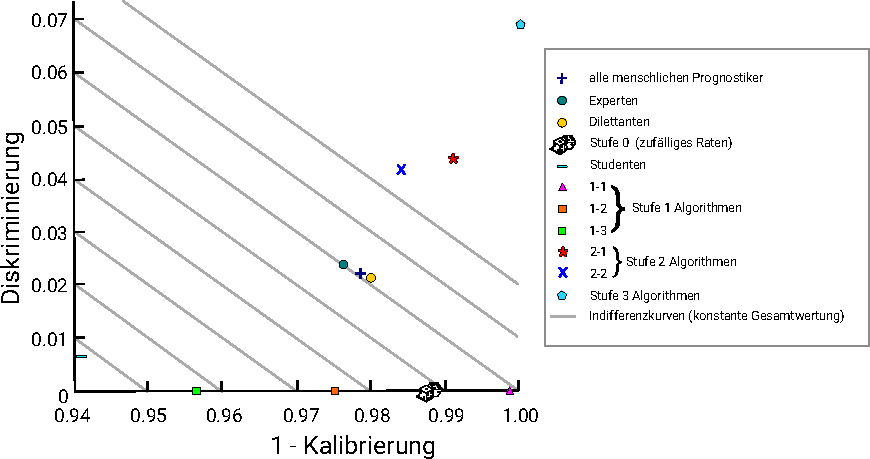
\includegraphics[scale=1.0]{Grafiken/Tetlock_1_Fertig_Ink.pdf} 
\label{pic:Tetlock_1}
\end{figure}
Die zwei
Bestandteile des \emph{probability score}, Kalibrierung (\emph{calibration}) und
Diskriminierung (\emph{discrimination}), sind auf den Achsen abgebildet. \\ \\ 
Kalibrierung (horizontale Achse) misst die Fähigkeit eines Prognostikers,
Ereignisse korrekt nach ihrer
Auftrittswahrscheinlichkeit zu ordnen (vgl. \cite{Tetlock}, S.~47). So ist ein
Prognostiker gut kalibriert, wenn etwa 10~\% der Ereignisse eintreten, für die
er eine Wahrscheinlichkeit von 0.1 geschätzt hat, 20~\% der Ereignisse eintreten
die eine Wahrscheinlichkeit von 0.2 erhalten haben, und so weiter. Je kleiner
der numerische Wert der Kalibrierung, desto besser ist der Prognostiker. Bei
einem Wert von 0 ist die bestmögliche Kalibrierung erreicht und aus diesem Grund
ist (1 - Kalibrierung) auf der horizontalen Achse abgebildet. \\ \\
Weiterhin ist ein Prognostiker umso besser bei der Diskriminierungskomponente
(vertikale Achse),
je eher es ihm gelingt die Auftrittswahrscheinlichkeiten von einzelnen
Ereignissen von der relativen Häufigkeit aller Ereignisse\footnote{
genauer: Das Verhältnis der Anzahl der eingetretenen Ereignisse zu der
Gesamtanzahl der Ereignisse} (\emph{base-rate})
zu unterscheiden. Perfekte Diskriminierung wird erreicht, wenn allen 
eingetretenen Ereignissen eine Wahrscheinlichkeit von 1.0 zugeordnet wird, und
alle Ereignisse, die nicht eingetreten sind, mit Null bewertet werden
(vgl. \cite{Tetlock}, S.~47).\\ \\
Nun gehen Kalibrierung und Diskriminierung als Summe in den
\emph{probability score} ein. Aus diesem Grund kann sich für verschiedene
Werte von Kalibrierung und Diskriminierung der gleiche Wert für den
\emph{probability score} ergeben. Die diagonalen Linien in Abbildung~\xcom
markieren Stellen mit konstantem \emph{probability score}. Je weiter rechts oben
eine Linie verläuft, desto höher ist der zugehörige \emph{probability score}.
\\ \\
Die Gesamtergebnisse für Kalibrierung und Diskriminierung für die verschiedenen
Teilnehmergruppen sind in der Graphik eingetragen. Die am besten qualifizierte
Gruppe stellen die Experten dar, die Fragen zu ihren jeweiligen Fachgebieten
erhalten haben (vgl. \cite{Tetlock}, S.~242). Weniger qualifiziert sind die 
\glqq{Dilettanten}\grqq (\emph{dilettantes}), Experten, die jedoch Fragen
beantwortet haben, die nicht zu ihrem Spezialgebiet gehören. Die Dilettanten
gaben an, dass sie sich mit Hilfe qualititativ hochwertiger Quellen
(\emph{Economist}, \emph{Wall Street Journal}, \emph{New York Times} etc.) über
Themen außerhalb ihrer Fachgebiete informieren (vgl. \cite{Tetlock}, S.~56).
Die Gruppe mit der geringsten Qualifikation waren Studenten, die die Übungen
zu Vorhersagen absolvieren mussten, nachdem sie kurze Zusammenfassungen von
Fakten zu den jeweiligen Themen erhalten haben (vgl. \cite{Tetlock}, S.~56).
\\ \\
Weiterhin enthält Abbildung~\ref{pic:Tetlock_1} auch die Ergebnisse, die von den
statistischen Algorithmen erzielt wurden. Zur besseren Übersicht werden die
Algorithmen hier in vier Gruppen eingeteilt. Der Stufe 0 Algorithmus würfelt
einfach die Antworten , er ordnet den zur Debatte stehenden Ereignissen
zufällige Wahrscheinlichkeiten zu. Weiterhin gibt es mehrere Varianten von
Stufe 1 Algorithmen, die als Antwort auf die Fragen immer die relative
Häufigkeit der Ereignisse eintragen. Etwas komplexer sind die Stufe 2
Algorithmen. Diese extrapolieren aus der Vergangenheit in die Zukunft und setzen
die Wahrscheinlichkeiten für die Ereignisse entsprechend. Die höchste
Komplexität hat der Stufe 3 Algorithmus. Um die Eintrittswahrscheinlichkeiten
der Ereignisse zu ermitteln, nutzt dieser die Vergangenheitswerte mehrerer
Variablen, die eine hohe Vorhersagekraft besitzen.\footnote{Die genaue Zuordnung
der Stufen 0-3 zu den Algorithmen in der Originalquelle (\cite{Tetlock}, S.~51)
sieht folgendermaßen aus:
\begin{description}
\item[Stufe 0:] \emph{random guessing} (\emph{chimp})
\item[Stufe 1:] \emph{contemporary base rate} (1-1), \emph{restrictive base
  rate} (1-2), \emph{expansive base rate} (1-3)
\item[Stufe 2:] \emph{cautious case-specific extrapolation} (2-1),
  \emph{aggressive case-specific extrapolation} (2-2)
\item[Stufe 3:] \emph{autoregressive distributed lag models}
\end{description}
} \\ \\
Abbildung~\ref{pic:Tetlock_1} zeigt, dass die Experten die Studenten bei
den \emph{forecasting exercises} deutlich schlagen konnten. Allerdings waren die
Experten kaum besser (!) als der zufallsgesteuerte Algorithmus 
(Stufe 0)\footnote{Die Experten waren schlechter kalibriert aber besser bei
der Diskriminierung, sodass sie insgesamt eine etwas bessere Gesamtwertung
hatten}. Insbesondere verloren die Experten gegen die komplexeren Algorithmen
(Stufe 2 und 3) mit deutlichem Abstand und zwar sowohl bei Kalibrierung, als
auch bei Diskriminierung. Falsche Überzeugungen und mentale Barrieren haben, so
Tetlock, das Urteilsvermögen der Experten getrübt und zu den schlechten
Ergebnissen geführt (mehr dazu in Abschnitt~\xcom). \\ \\
Was haben diese Ergebnisse mit \emph{predictive analytics} und dem öffentlichen
Sektor zu tun?\\ \\
Erstens waren die Fragestellungen der \emph{forecasting exercises} aus den
Bereichen Politik und Wirtschaft\footnote{
Andere Themen, wie beispielweise naturwissenschaftliche Fragestellungen,
z. B. \glqq{Wie} wahrscheinlich ist die Detektion dunkler Materie
in den nächsten fünf Jahren?\grqq, wurden nicht behandelt.
}, was für den öffentlichen Sektor relevant ist. Zweitens handelt es sich dabei
um generelle Probleme der menschlichen Urteilsfindung. Probleme, die in vielen
Bereichen auftreten und zu Fehleinschätzungen führen können. Zudem
konnten datenbasierte Algorithmen, also \emph{predictive analytics}, die
menschlichen Vorhersagen bei den \emph{forecasting exercises} schlagen. Dies
deutet darauf hin, dass formale Methoden wie \emph{predictive analytics} dabei
helfen können, bessere Urteile zu fällen und folglich auch bessere
Entscheidungen zu treffen. \\ \\
Der nächste Teil der Arbeit behandelt \emph{predictive analytics},
den Prozess der (menschlichen) Urteilsfindung und wie formale Methoden diesen
Prozess verbessern können.
